% !TEX encoding = UTF-8 Unicode
% !TEX TS-program = pdflatex

%%%%%%% La riga soprastante serve per configurare gli editor
%%%%%%% TeXShop, TeXworks e TeXstudio per gestire questo file
%%%%%%% con la codifica UFF-8.
%%%%%%% Se si vuole usare un'altra codifica si veda sotto.
%%%%%%%

%%%%%%%  Esempio con molte opzioni
%%%%%%% Le opzioni nella forma "chiave=valore" sono definite
%%%%%%% perché la classe dalla versione 6.1.00 usa il pacchetto
%%%%%%% xkeyval. Vedere sulla documentazione in inglese o
%%%%%%% in italiano quali chiavi accettano valori.

%%%%%%% L'opzione per il corpo accetta qualsiasi valore, anche fratto
%%%%%%% (per esempio: corpo=11.5pt) e va sempre scritto con una
%%%%%%% unità di misura. L'utente è pregato di non esagerare con
%%%%%%% corpi normali minori di 9.5pt o maggiori di 13pt.
%%%%%%%
%%%%%%% Le opzioni per inputenc e fontenc vanno per prime.
%%%%%%% Vengono ignorate se NON si compone con pdfLaTeX. Ma
%%%%%%% questo è un esempio per pdfLaTeX.
%%%%%%%

 \documentclass[%
    corpo=12pt,
    twoside,
%    stile=classica,
    oldstyle,
%    autoretitolo,
    tipotesi=magistrale,
    greek,
    evenboxes,
    english
]{toptesi}
%%%%%%%%%%%%%%%%%%%%%%%%%%%%%%%%%%%%%%%%%%%%%%%%%%%%
%%%%%% Per la codifica d'entratasi può scegliere quella che si vuole,
%%%%%% ma si consiglia di preferire utf8; in ogni caso non scegliere
%%%%%% codifiche specifiche del sistema operativo.

\usepackage[utf8]{inputenc}% codifica d'entrata
\usepackage[T1]{fontenc}%    codifica dei font
\usepackage{lmodern}%        scelta dei font

% Vedere la documentazione toptesi-it.pdf per le
% attenzioni che bisogna usare al fine di ottenere un file
% veramente conforme alle norme per l'archiviabilità.


\usepackage[hidelinks]{hyperref}

\hypersetup{%
	pdfauthor={Gabriele Degola},
    pdfpagemode={UseOutlines},
    bookmarksopen,
    pdfnewwindow=true,
    pdfstartview={FitH}
  }
%
%%%%%%% Esempio di composizione di tesi di laurea con PDFLATEX 
%
\usepackage{lipsum}
\usepackage{subcaption}
\usepackage{biblatex}
\addbibresource{references.bib}
\usepackage[acronym]{glossaries}
%

\makeglossaries
\newacronym{ai}{AI}{artificial intelligence}
\newacronym{ilsvrc}{ILSVRC}{ImageNet Large Scale Visual Recognition Challenge}
\newacronym{cnn}{CNN}{Convolutional Neural Network}
\newacronym{svm}{SVM}{Support Vector Machines}
\newacronym{ide}{IDE}{Integrated Development Environment}
\newacronym{iou}{IoU}{Intersection over Union}
\newacronym{roc}{ROC}{Receiver Operating Characteristic}
\newacronym{auc}{AUC}{Area Under the Curve}
\newacronym{ap}{AP}{Average Precision}
\newacronym{map}{mAP}{mean Average Precision}
\newacronym{json}{JSON}{JavaScript Object Notation}
\newacronym{xml}{XML}{Extensible Markup Language}
\newacronym{voc}{VOC}{Visual Object Classes}
\newacronym{kitti}{KITTI}{Karlsruhe Institute of Technology and Toyota Technological Institute}
\newacronym{rcnn}{R-CNN}{region-based Convolutional Neural Network}
\newacronym[firstplural=Regions of Interest (RoIs)]{roi}{RoI}{Region of Interest}
\newacronym{rpn}{RPN}{Region Proposal Network}
\newacronym{fpn}{FPN}{Feature Pyramid Network}
\newacronym{ssd}{SSD}{Single Shot Detector}
\newacronym{yolo}{YOLO}{You Only Look Once}
\newacronym{adda}{ADDA}{Adversarial Discriminative Domain Adaptation}
\newacronym{dann}{DANN}{Domain Adversarial Neural Network}
\newacronym{coco}{COCO}{Common Objects in Context}
\newacronym[firstplural=GPUs]{gpu}{GPU}{Graphics Processing Unit}
\newacronym{cpu}{CPU}{Central Processing Unit}

\glsdisablehyper

%%%%%%% Definizioni locali
\newtheorem{osservazione}{Osservazione}% Standard LaTeX
\ExtendCaptions{english}{Abstract}{Acknowledgements}

\begin{document}\errorcontextlines=9
%%%%%%% Questi comandi è meglio metterli dentro l'ambiente
%%%%%%% ThesisTitlePage con o senza asterisco, oppure in un file di
%%%%%%% configurazione personale. Si veda la documentazione
%%%%%%% inglese o italiana.
%%%%%%% Comunque i presenti comandi servono per comporre la
%%%%%%% tesi con i moduli di estensione standard del pacchetto
%%%%%%% TOPtesi.

\english

\begin{ThesisTitlePage}*
% Per cambiare la dicitura sopra la lista dei laureandi decommentare
% la riga seguente, cambiando le 4 parole in modo consistente
%
%\TitoloListaCandidati{Studente,Studenti,Studentessa,Studentesse}
%
\ateneo{Politecnico di Torino}
%
% Non tutte le università hanno un nome proprio
\nomeateneo{Dipartimento di Automatica e Informatica}
%
\titolo{Domain Adaptation for Object Detection}% per la laurea quinquennale e il dottorato
\sottotitolo{A data augmentation approach}% per la laurea quinquennale e il dottorato
%
%%%%%%% Corso degli studi
\CorsoDiLaureaIn{Master Degree in}
\corsodilaurea{Data Science and Engineering}% per la laurea

\TesiDiLaurea{Master Degree Thesis}

%%%%%%% L'eventuale numero di matricola va fra parentesi quadre
%\show\Candidato
%\def\Candidato{Studente}
%\show\Candidato
\CandidateName{Candidate}
\candidato{Gabriele \textsc{Degola}}
%\secondocandidato{Evangelista \textsc{Torricelli}}[123457]

%%%%%%% Relatori o supervisori
%
\AdvisorName{Supervisor}
\relatore{prof.~Paolo \textsc{Garza}}
% 
%%%%%%% Per mettere altri relatori consultare toptesi-it.pdf

%%%%%%% Tutore
%\tutoreaziendale{dott.\ ing.\ Giovanni Giacosa}
%\NomeTutoreAziendale{Supervisore aziendale\\Centro Ricerche FIAT}

%%%%%%% Seduta dell'esame
%\sedutadilaurea{Agosto 1615}
%%%%%%%% oppure:
\sedutadilaurea{\textsc{Academic~Year} 2021-2022}% 

%%%%%%% Logo della sede
\logosede[4cm]{logopolito}% 
\end{ThesisTitlePage}

\sommario



% \paginavuota % funziona anche senza specificare l'opzione classica

\ringraziamenti



\tablespagetrue\figurespagetrue % normalmente questa riga non serve ed e' commentata
\indici

\mainmatter

\chapter*{Introduction}

\chapter{Related works}

\section{Object detection}
Object detection methods are able to recognize the objects represented in an image and to highlight their position, returning the associated bounding boxes, rectangular boxes which contain an object. The bounding box format depends on the model and on the dataset. Typically, they are determined by the \textit{x} and \textit{y} coordinates of the upper-left corner
%, as in \acrshort{coco} (\ref{sec:coco}),
or of the center
%, as in \acrshort{yolo} (\ref{sec:yolo}),
and by the bounding box width and height.

\begin{figure}[ht]
	\centering
	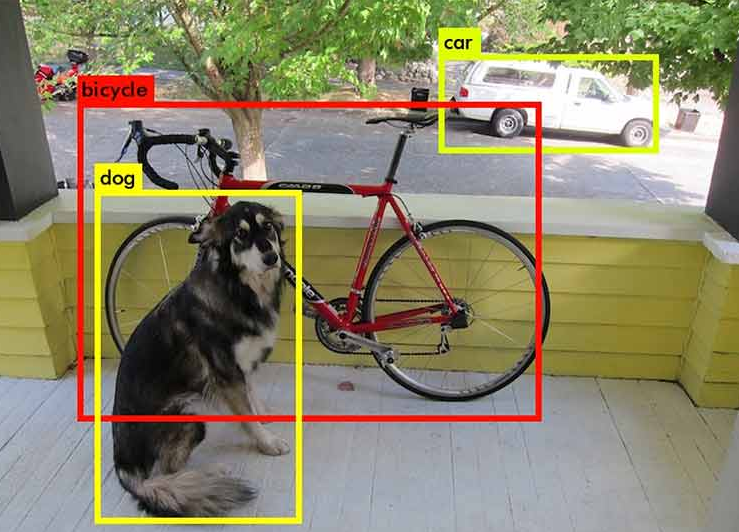
\includegraphics[width=.5\textwidth]{imgs/yolo_detection.png}
	\caption{An example of object detection\cite{redmon2016look}}
\end{figure}

Object detection is a fundamental task in modern computer vision, with applications such as autonomous driving, robot vision and human-computer interaction.

\subsection{Existing methods}
An object detection task can be seen as a combination of two main steps: finding image regions that may contain objects, and then independently classifying the objects in those regions. Before deep learning, this was achieved using a sliding-window approach, where an image classifier was applied to different areas of the image and only the predictions with the highest probability were retained. Nowadays, two main families of object detectors can be identified.

\subsubsection{Two stage object detectors}
As said, the most commonly used models for object detection are based on a two-stage approach and belong to the family of \glspl{rcnn}. In basic \acrshort{rcnn}\cite{girshick2014rich}, a manageable number of possible \glspl{roi} are extracted from an image and a \gls{cnn} is evaluated independently on each \acrshort{roi} to extract features that are fed into a \gls{svm} to classify the presence of an object in that region and the bounding box location. Fast \acrshort{rcnn}\cite{girshick2015fast} and Faster \acrshort{rcnn}\cite{ren2016faster} improved the region selection algorithm, analysing only interesting \glspl{roi} and exponentially reducing the inference time. Because of its good performances and speed, Faster \acrshort{rcnn} is widely used for benchmarking and as base for several derived works.


The main contribution of Faster \acrshort{rcnn} is the introduction of a \gls{rpn}, which integrate some convolutional layers of the image classifier into the region proposal phase. That allows the network to be trained in an end-to-end fashion.

\begin{figure}[ht]
	\centering
	\subcaptionbox{Description of \acrshort{rcnn}\cite{girshick2014rich}}{
		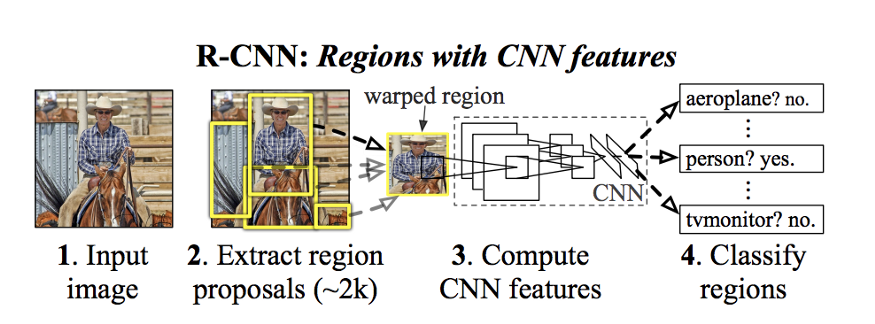
\includegraphics[width=.6\linewidth]{imgs/rcnn.png}
	}
	\subcaptionbox{Description of Faster \acrshort{rcnn}\cite{ren2016faster}}{
		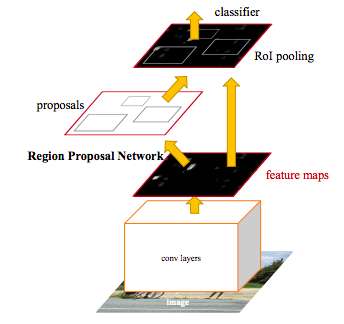
\includegraphics[width=.3\linewidth]{imgs/fasterrcnn.png}
	}
	\caption{Architecture of two stage object detectors}
	\label{fig:architectures}
\end{figure}

\subsubsection{One stage object detectors}
Differently from two stage detectors, one stage object detectors skip the region proposal step and focus on predicting object regions and classes together. This leads to faster predictions with respect to two stage models, making them suitable for real-time applications at the cost of lower prediction quality. The pioneer work for one stage object detection is OverFeat\cite{sermanet2014overfeat}, published in 2014. Here, the last classification layers of a standard \gls{cnn} are replaced by a regression network for each class, in order to predict the object bounding boxes.

\paragraph{YOLO}\label{sec:yolo}
The \acrfull{yolo} model\cite{redmon2016look} uses pretrained \gls{cnn} for classification and splits each image in cells. If the center of an object falls into a cell, that cell is responsible for detection and should predict the bounding box locations, a confidence score and a class probability for the detected objects. A specific loss function is used to efficiently learn at the same time to predict bounding boxes and object classes.

\paragraph{SSD}
\acrfull{ssd}\cite{Liu_2016} adds several convolutional layers of decreasing sizes, in order to build a \textit{pyramid representation} of the images and efficiently detect object of different sizes, at each pyramidal layer. Instead of splitting images in cells, anchor boxes are used for faster detection.

\begin{figure}
	\centering
	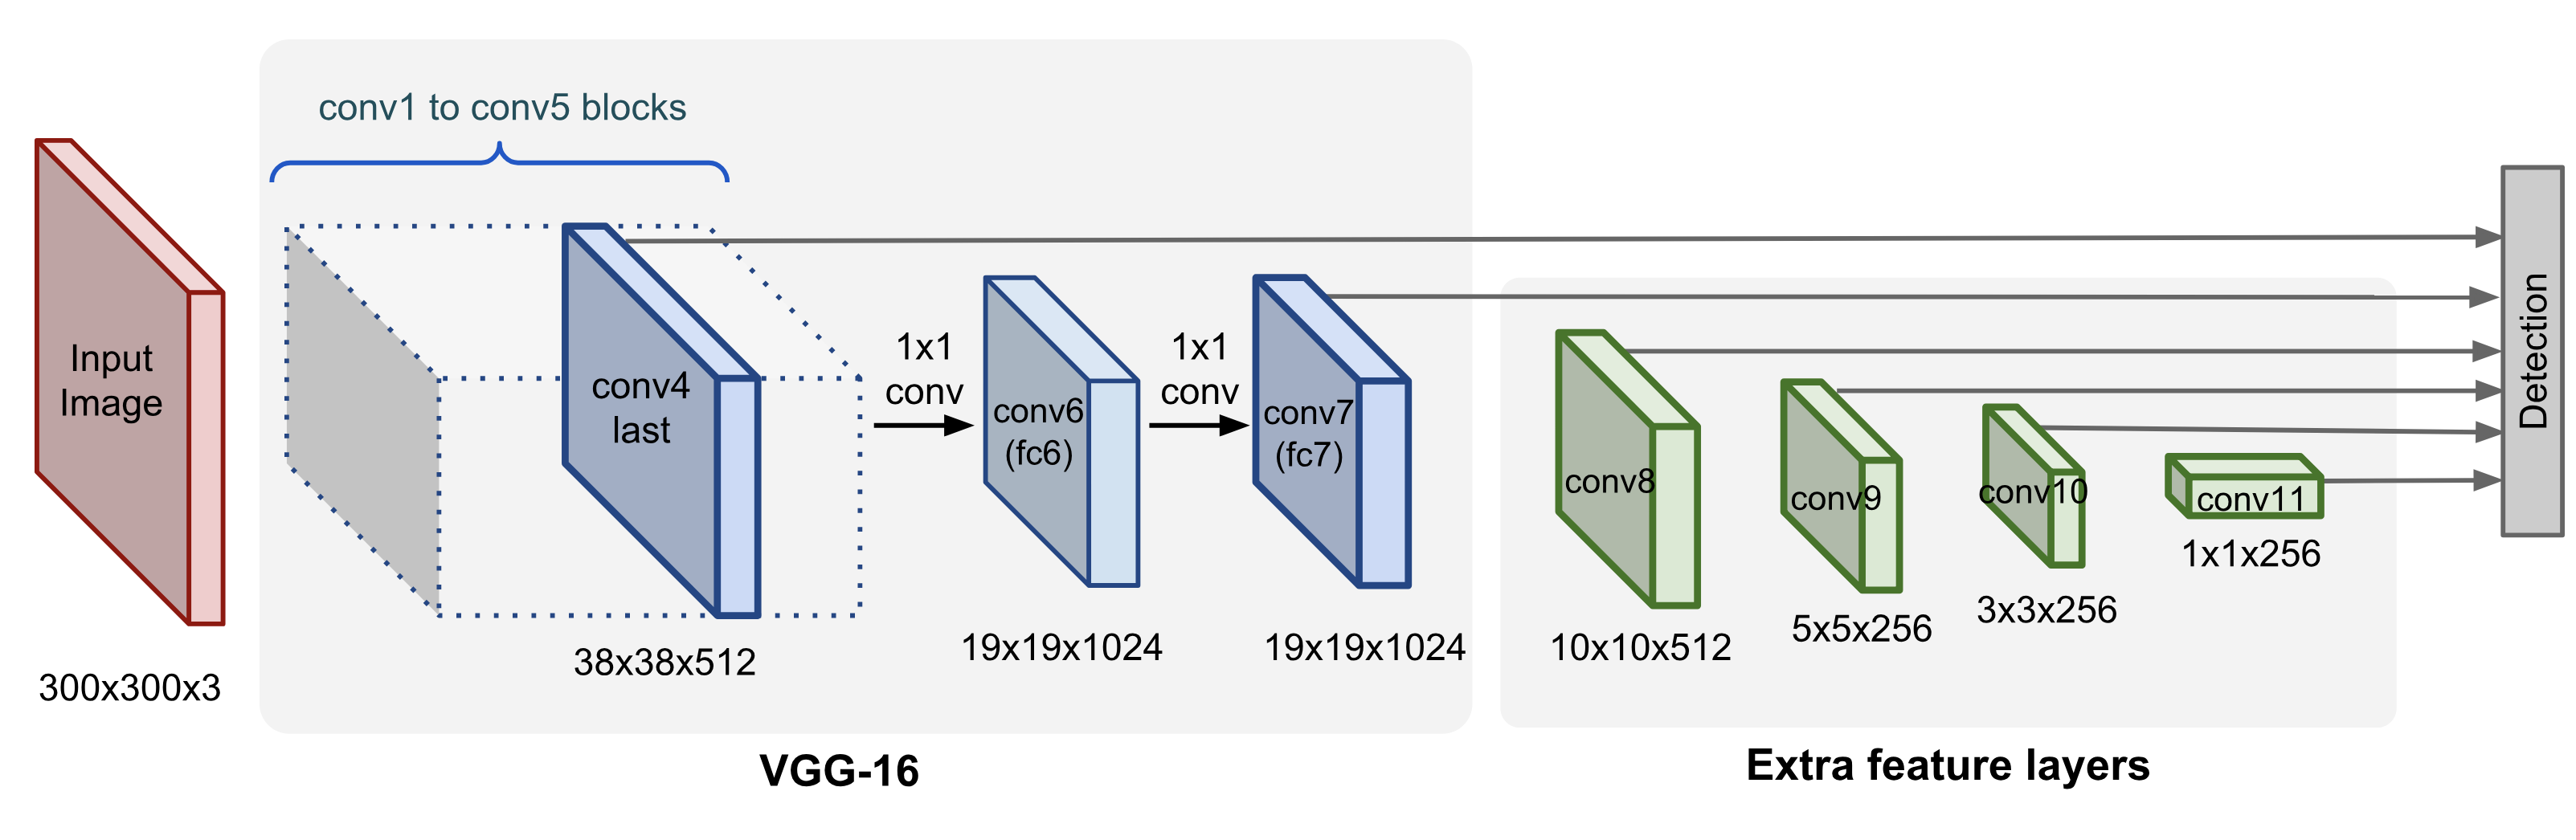
\includegraphics[width=.7\linewidth]{imgs/SSD-architecture.png}
	\caption{\acrshort{ssd}'s pyramid architecture\cite{objdetpart4}}
	\label{fig:ssd}
\end{figure}

\paragraph{RetinaNet}
The main improvements of RetinaNet\cite{lin2018focal} over previous one stage detection model are the use of \textit{feature pyramid network} as part of the backbone and of \textit{focal loss}, which helps to approach the results of two-stage detectors.

\begin{figure}[ht!]
	\centering
	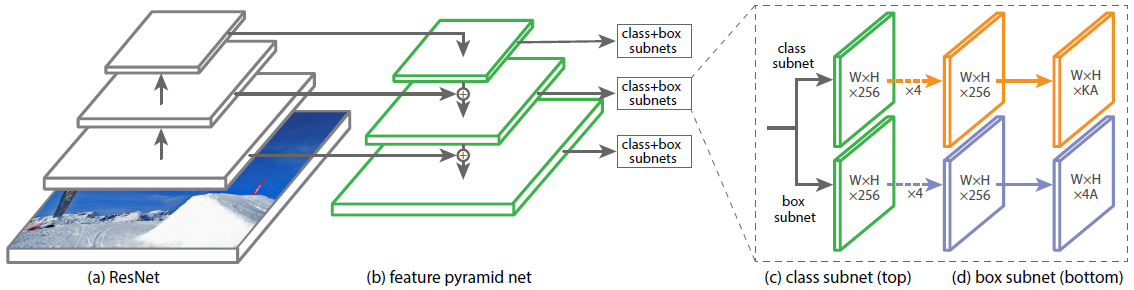
\includegraphics[width=0.8\linewidth]{imgs/retinanet.png}
	\caption{RetinaNet architecture\cite{lin2018focal}}
	\label{fig:retinanet}
\end{figure}

\subparagraph{Feature pyramid network}
\glspl{fpn}\cite{lin2017feature} adopt and improve the same approach as \acrshort{ssd}'s pyramid layers. They are composed by a sequence of pyramid levels which correspond to network stages. Each stage is composed by multiple convolutional layers of the same size, divided by two at consecutive stages. In addition to standard feedforward, different stages are linked by a top-down pathway in the opposite direction and lateral connections. This allows the network to construct a rich and multi-scale feature pyramid for each input image.

After their proposal in the context of single-stage detectors, the \glspl{fpn} have also been used as part of the backbone of two-stage detectors, to improve their performance.

\subparagraph{Focal loss}
One of the main obstacles for the training of  other object detector models is the large imbalance between background and foreground examples, which drives the model to focus on irrelevant background regions.

The focal loss, introduced by RetinaNet, is based on the \textit{cross entropy} loss. For binary classification, the cross entropy loss is widely used and defined as:
\begin{center}
	$CE(p,y) = \begin{cases}
		-\log(p) & \text{if $y$ = 1}\\
		-\log(1-p) & \text{otherwise.}
	\end{cases}$
\end{center}
where $y\in \{\pm 1\}$ is the ground truth class and $p\in\left[0,1\right]$ is the model's probability for class $1$. Defining $p_t$ as:
\begin{center}
	$p_t = \begin{cases}
		p & \text{if $y$ = 1}\\
		1-p & \text{otherwise.}
	\end{cases}$
\end{center}
cross entropy can be written as $CE(p,y) = CE(p_t) = -\log(p_t)$.

\bigskip
A balanced version of the cross entropy loss is sometimes used to deal with class imbalance. A numeric factor $\alpha\in\left[0,1\right]$ can be introduced for class $1$, with value $1-\alpha$ for class $-1$. $\alpha_t$ is defined analogously to $p_t$. Therefore, the balanced cross entropy is written as:
\begin{center}
	$CE(p,y) = -\alpha_t\log(p_t)$.
\end{center}

\bigskip

\section{Domain adaptation}

%\blankpagestyle{headings}

%\lipsum[1-2]

\chapter{Method}

\chapter{Experiments and results}

\chapter*{Conclusions}

\backmatter
\printbibliography[heading=bibintoc]


\end{document}
